\chapter{Configuring Your MEGA65}

\section{Configuring Your MEGA65}
\label{cha:configuringyourmega}
\index{Configuration}

This chapter describes how to configure your MEGA65.

Configuration data is stored on the SD card, so this chapter also describes how to prepare a new SD card. Your MEGA65 comes with an SD card pre-installed. If you configure your MEGA65 using the pre-installed SD card then later install a new SD or microSD card, you will need to set your configuration settings again.

This chapter also introduces the MEGA65 Filehost website, which you can use to download games, apps, tools, and system updates for your computer.

\section{The Configuration Utility}
\label{sec:configuration-utility}
\index{Configuration!Utility}

You can configure your MEGA65 using the Configuration Utility. This includes the settings shown when you switched on the machine for the first time, and many others.

To access the Configuration Utility, switch off the MEGA65, hold the \specialkey{ALT} key and switch it back on. The Utility menu\index{Utility menu} appears with several options. Press \megakey{1} to start the Configuration Utility.

\begin{center}
  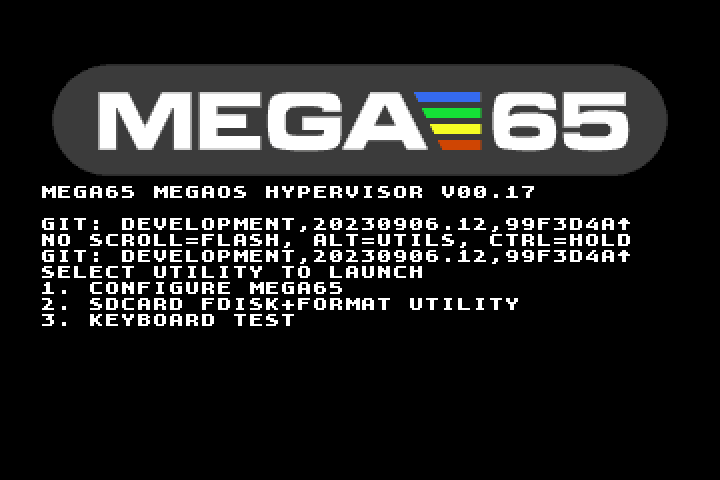
\includegraphics[width=0.7\linewidth]{images/ss-utilmenu.png}
\end{center}

The Configuration Utility includes several pages of settings, which you can navigate using the keyboard or a mouse connected to port 1. Use \megakey{$\leftarrow$} and \megakey{$\rightarrow$} to navigate between pages, and \megakey{$\uparrow$} and \megakey{$\downarrow$} to select items on the page. Press \specialkey{RETURN} or \megakey{SPACE} to toggle a setting or change a value.

\subsection{Input}
\index{Configuration!Mouse}

The {\bf Input} page configures the mouse settings for the two peripheral ports.

\begin{center}
  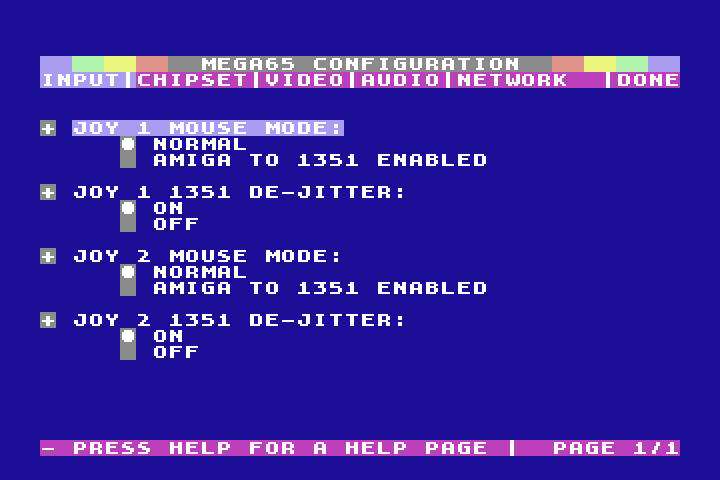
\includegraphics[width=0.7\linewidth]{images/ss-m65config-1.png}
\end{center}

The MEGA65 supports the Commodore 1351 mouse,\index{Commodore 1351 mouse} the Commodore Amiga mouse,\index{Commodore Amiga mouse} or modern equivalents such as a USB mouse connected with a \href{https://retrohax.net/shop/amiga/mouster/}{mouSTer} adapter.\index{mouSTer adapter} The port must be set to the correct mouse type, where {\bf normal} refers to the 1351 mouse. If an Amiga mouse is connected while the port is in the {\bf normal} mode, it may interfere with the behaviour of the keyboard.

The {\bf 1351 De-jitter} setting adjusts the sensitivity in Commodore 1351 mouse mode to avoid jitter in the mouse pointer. It is recommended to leave this set to {\bf on} when using a 1351 mouse in {\bf normal} mode.

\subsection{Chipset}
\index{Configuration!Boot Disk}

The {\bf Chipset} page configures several features, including the Real-Time Clock.

\begin{center}
  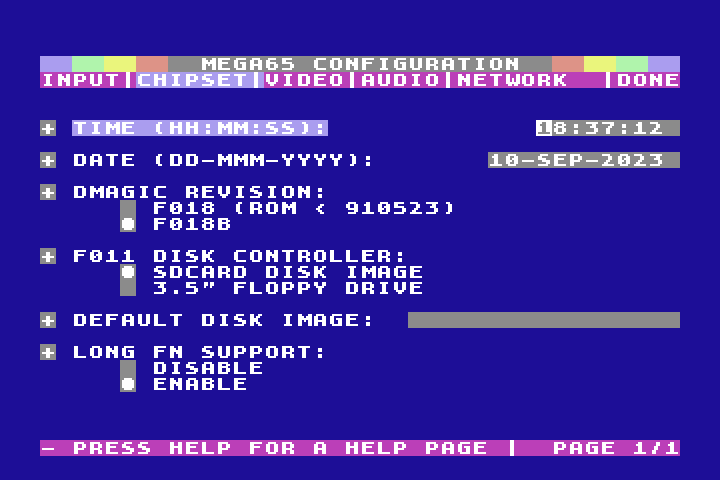
\includegraphics[width=0.7\linewidth]{images/ss-m65config-2.png}
\end{center}

To set the Real-Time Clock, select the time or date field, type the complete value, then press \specialkey{RETURN}.\index{Real-Time Clock!Setting the Date/Time}\index{Configuration!Real-Time Clock} The clock setting takes effect as soon as you press \specialkey{RETURN}, and does not take effect unless you press \specialkey{RETURN}. Note that all other settings are not saved until the end. Only the RTC is updated immediately.

The {\bf DMAGIC revision} field controls the behavior of the DMA controller. In most cases, you want the newer {\bf F018B} setting. The {\bf F018} setting is for backwards compatibility when running the C65 versions of the ROM, and is not always required.

The {\bf F011 disk controller}\index{F011 Disk Controller} field determines whether the MEGA65 looks for a boot disk on the SD card or in the physical 3.5" floppy drive when the computer is switched on.\index{Configuration!Boot Disk} When set to {\bf SDCARD disk image,} the MEGA65 uses the D81 virtual disk image named in the {\bf default disk image} field as the boot disk. When you first get your MEGA65, this is set to the Intro Disk,\index{Intro Disk} named {\tt MEGA65.D81}. You can change this to a different disk. To disable auto-mounting, change the disk name to a filename that does not exist, or rename the {\tt MEGA65.D81} file on the SD card. (Leaving the setting empty will default to {\tt MEGA65.D81}.)

If {\bf F011 disk controller} is set to {\bf 3.5" floppy drive,} the boot process will pause just before the \screentext{READY} prompt to check if a boot disk is inserted in the drive. If you do not use a physical boot disk, you may wish to leave this set to {\bf SDCARD disk image} for a faster boot process.

{\bf Long FN support} refers to long filename support in the MEGA65 SD card file browser features. Leave this enabled unless there is an issue with reading files with filenames longer than 11 characters.

\subsection{Video}
\index{Configuration!Video}

The {\bf Video} page configures video settings. These are the same settings from the on-boarding configuration, including the PAL or NTSC video mode, Digital Video sound, and CRT emulation.\index{Configuration!On-boarding}\index{Display!Setting PAL/NTSC}

\begin{center}
  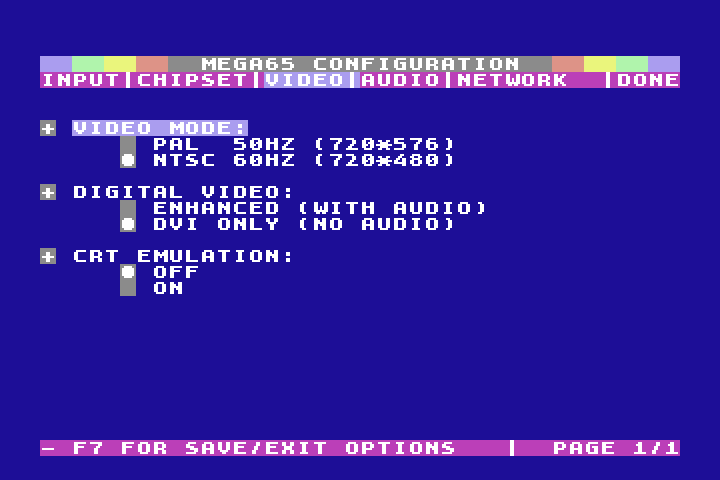
\includegraphics[width=0.7\linewidth]{images/ss-m65config-3.png}
\end{center}

{\bf Video mode} selects between the PAL compatibility mode and the NTSC compatibility mode. You can also change this while running programs using the Freezer menu.

The {\bf Digital Video} setting enables or disables the combined video and audio signal over the Digital Video port. If your Digital Video display has built-in speakers, enable this setting ({\bf Enhanced (with audio)}) to use them. Some DVI displays without built-in speakers require that this is disabled.

{\bf CRT emulation} is an optional setting that makes the picture look more like that of a vintage Cathode Ray Tube display when using a modern flat-panel display.

\subsection{Audio}
\index{Configuration!Audio}

The {\bf Audio} page configures the MEGA65 sound system.\index{Configuration!Audio} In most cases, you can leave these at their default settings.

\begin{center}
  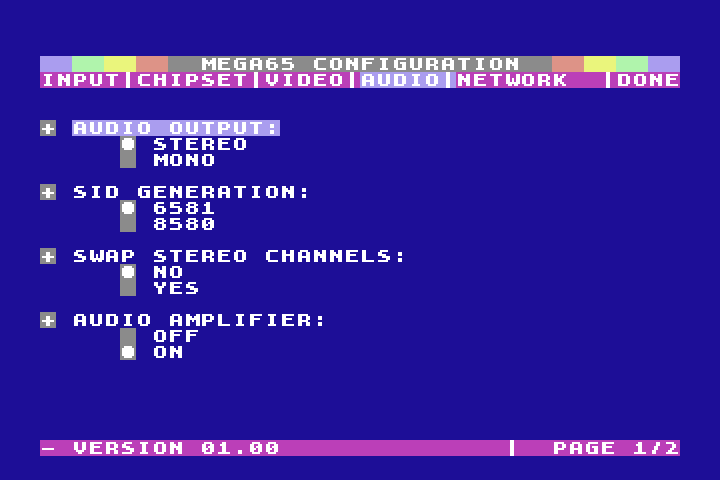
\includegraphics[width=0.7\linewidth]{images/ss-m65config-4.png}
\end{center}

{\bf Audio output} can be configured to use full stereo, or to send a monoaural signal to both speakers. When in stereo mode, various audio devices in the MEGA65 can be panned to the left or right using the audio mixer in the Freezer menu. The default settings pan the four SID chips slightly to the left and right.

{\bf SID generation} selects between the audio emulation of the two models of SID sound chips: the original 6581 used in some Commodore 64s, and the newer 8580 used in later Commodore 64s and 128s. Some Commodore 64 games took advantage of flaws in the 6581 that were fixed in the 8580, and so sound better with the older generation.

{\bf Swap stereo channels} switches the stereo mix to use the opposite speakers.

{\bf Audio amplifier} controls the built-in amplifier on the 3.5 mm audio jack. Set this to {\bf on} when using headphones or another device that expects an amplified signal. Set this to {\bf off} for a line-level signal.

\subsection{Network}
\index{Configuration!Network}

The {\bf Network} page gives you the opportunity to adjust the MAC address of the Ethernet port. The MEGA65 does not have a hardware-assigned MAC address. Instead, it uses the value entered here.

If the MAC address is set to all zeros, press the \megakey{R} key to generate a random address. Networking features will not function with a MAC address set to all zeros.\index{Configuration!MAC address}\index{Networking!MAC address}

\begin{center}
  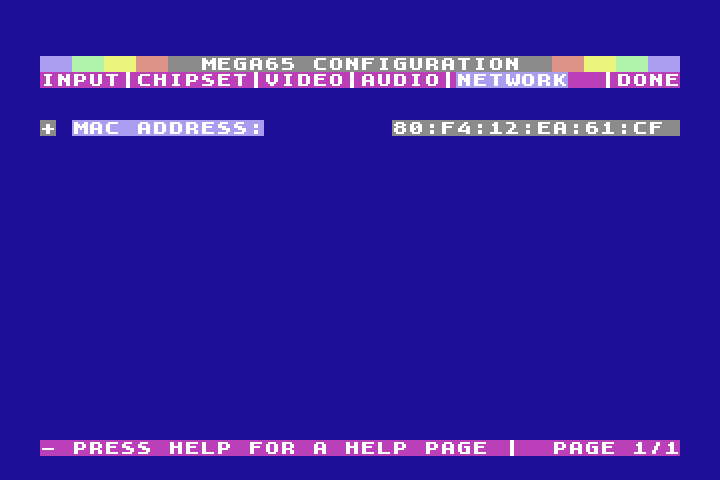
\includegraphics[width=0.7\linewidth]{images/ss-m65config-5.png}
\end{center}

\subsection{Done}

The {\bf Done} page lets you exit the Configuration Utility. If you have made changes that you want to keep, select {\bf Save as defaults and exit.} You can also abandon changes, restore the factory default settings, or completely restart to the on-boarding screen.

\begin{center}
  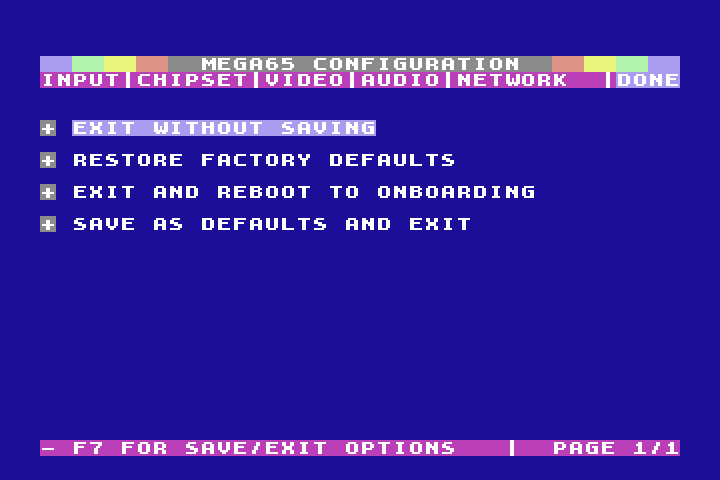
\includegraphics[width=0.7\linewidth]{images/ss-m65config-save.png}
\end{center}

When you exit the Configuration Utility, you will be prompted to ``power-cycle'' the computer. Switch the computer off, then switch it on again.

\section{Introducing SD Cards}
\label{sec:introducing-sd-cards}
\index{SD Cards}
\nopagebreak
Your MEGA65 is equipped with two SD card slots: a full-size SD card slot inside the case accessible from the bottom of the computer, and a microSD card slot accessible from the rear of the computer.\index{SD Cards!Locations} The MEGA65 uses the SD card for storing configuration settings, loading the operating system, updating the firmware, and storing your software and data as virtual disk images.

The MEGA65 includes a full-size SD card installed in the internal SD card slot, pre-populated with the operating system files and bundled software.\footnote{You can recreate the original SD card's contents using files that you can download from the Internet. Nevertheless, you may wish to make a backup of the SD card contents onto your PC.} You can connect your MEGA65 and start using it immediately without setting up a new SD card. You can leave this SD card in place and pretend that it isn't there, as if your MEGA65 is a computer from the 1990s, with a hidden ability to store non-volatile data.

The MEGA65 only uses one of the two SD card slots at one time. If there is a microSD card in the rear slot, the internal SD card is ignored. Which slot you use depends on how you expect to use the computer. As you get more familiar with your MEGA65, you may want to move the SD card between the MEGA65 and your PC to copy files and perform system updates. This is more convenient with the external microSD card slot.

Alternatively, you can connect your MEGA65 to your PC or local network with an Ethernet cable, and use a tool to transfer files between the two computers. The file transfer feature accesses files on the SD card, and uses whichever card slot is active. For more on transferring files, see chapter \vref{cha:transferring-files}.

\section{Preparing a New SD Card}

You can use the microSD memory card slot on the rear of the MEGA65 as persistent storage for the computer's configuration and system files. Having a prepared card in this slot overrides the SD card installed inside the computer. Having a microSD card installed is convenient if you wish to move it between your MEGA65 and your PC.

The following instructions apply to memory cards in either the external microSD card slot or the internal full-size SD card slot.

The MEGA65 supports SD cards of type SDHC, with sizes between 4GB and 32GB. Older cards smaller than 4GB and newer SDXC cards larger than 32GB are not expected to work.

An SD card must be prepared by the MEGA65 before use, using the SD Card Utility.\index{SD Card Utility} The utility creates two partitions: a hidden partition for configuration and freeze state data, and a FAT32-compatible partition for disk images and system files. You can access the FAT32 partition by connecting the SD card to your PC.\footnote{If you wish to make a backup of the complete SD card including the hidden partition, you must use a disk utility that copies entire partitions, not just the files on the FAT32 partition.}

An SD card formatted by another computer will {\em not} work with the MEGA65, even if it only erases the FAT32 partition. You {\em must} use the MEGA65 SD Card Utility to format the card.

\subsection{Inserting the SD Card}

Formatting an SD card erases its contents, and this operation cannot be undone. We recommend that you do not erase the internal SD card that came with the computer.

The SD Card Utility will prompt you to select which of the cards currently inserted in the computer to format. As a precaution, you may wish to remove the internal SD card before opening the SD Card Utility. You can reinstall it later, or leave it out of the machine until you need it. This is also a good opportunity to copy the bundled software files (with filenames that end in {\tt .D81}) off of the internal SD card to your PC, so they can be copied back to the new SD card later.

The utility menu is accessible even if no valid SD card is present. You can bootstrap a new system using just a compatible SD card and the SD Card Utility.

Insert the SD card that you wish to prepare before proceeding.

\subsection{The SD Card Utility}
\index{SD Card Utility}

You access the SD Card Utility from the Utility menu.\index{Utility menu} Switch off the MEGA65, hold the \specialkey{ALT} key and switch it on again. From the menu, select option \megakey{2} to start the SD Card Utility (\texttt{SDCARD FDISK+FORMAT UTILITY}).

\begin{center}
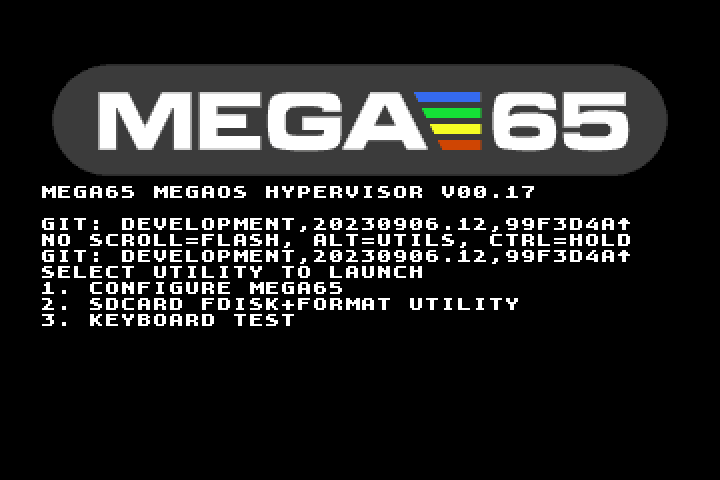
\includegraphics[width=0.7\textwidth]{images/ss-utilmenu.png}
\end{center}

The SD Card Utility opens and looks for SD cards installed in the slots. If you haven't inserted the SD card that you want to prepare yet, do so now, then press \megakey{R} to re-scan.

\begin{center}
  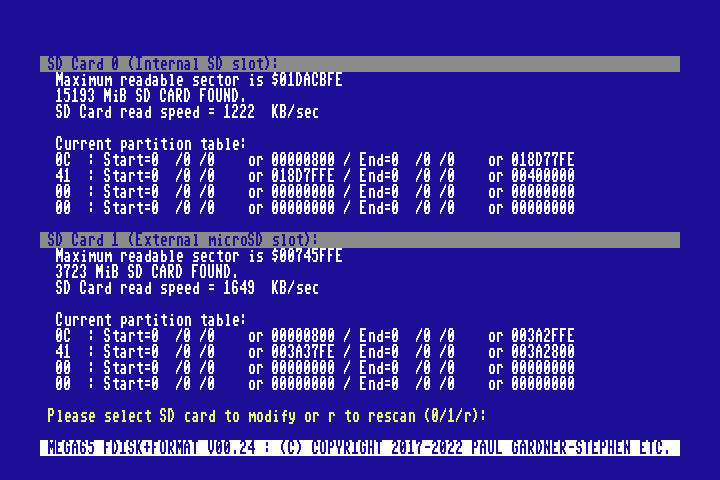
\includegraphics[width=0.7\textwidth]{images/ss-m65fdisk-busselect.png}
\end{center}

Select the card that you want to prepare: \megakey{0} for the internal SD card, \megakey{1} for the external microSD card. If you have two cards installed, {\em be careful to choose the correct card slot.}

The SD Card Utility prompts for confirmation to erase the SD card. As one last precaution, you must type the phrase {\tt DELETE EVERYTHING} in all capital letters, then press \specialkey{RETURN}, to proceed. (If you wish to abort this process, it is safe to switch off the MEGA65 at this time.)

\begin{center}
  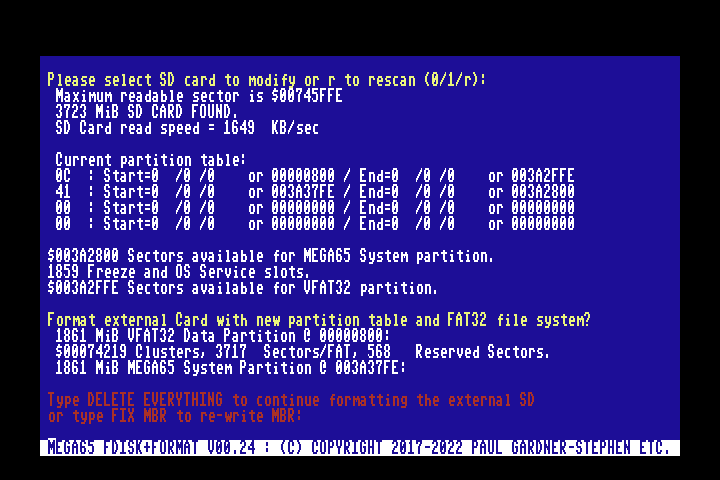
\includegraphics[width=0.7\textwidth]{images/ss-m65fdisk-typesomething.png}
\end{center}

The utility erases the SD card and sets up the partitions. When it is finished, it prompts to install the system files. The system files (with filenames ending in {\tt .M65} and {\tt .ROM}) are embedded in the core, and are copied to the FAT32 partition for use. If you have installed an updated MEGA65 core in slot 1, select it, otherwise select the factory-installed MEGA65 core in slot 0. (If you just received your MEGA65, slot 0 is the only option.)

\begin{center}
  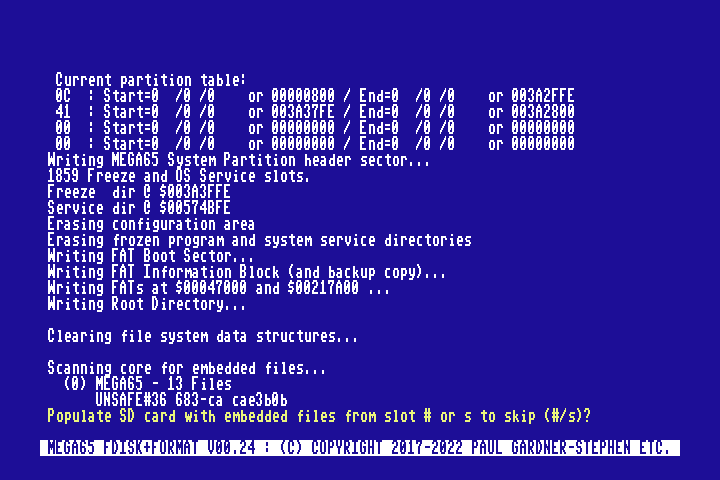
\includegraphics[width=0.7\textwidth]{images/ss-m65fdisk-populate.png}
\end{center}

When prompted, reboot the machine.\footnote{If you select a core that does not have {\tt MEGA65.ROM} as one of the embedded files, the utility will prompt you to move the SD card to your PC to copy this file onto it. This only happens when using a MEGA65 core from somewhere other than an official MEGA65 release package. For more information about cores and obtaining {\tt MEGA65.ROM}, see chapter \vref{cha:cores}.}

\subsection{Obtaining the Bundled Software}

The system files copied to the freshly formatted SD card do not include the bundled software that was included with the original SD card in the internal card slot. You can use your PC to copy these files off of the original SD card, then copy them back onto the new SD card.

The MEGA65 Filehost website\index{Filehost website} hosts all manner of files you can download for your MEGA65. This includes the latest versions of the platform components, alternate cores, and hundreds of games, demos, and applications produced by the MEGA65 community. This also includes the bundled software from the original SD card included with the computer.

If you no longer have the bundled software files, you can obtain them from the MEGA65 Filehost website. Visit the following URL:

\url{https://files.mega65.org/?id=all-intros-public}
